\subsection{Módulo de \textit{input}}

Os estados dos botões do GBA ficam salvos em um registrador. Cada um desses estados é representado por um \textit{bit} do valor guardado por esse registrador. Sempre que um botão é pressionado, o GBA automaticamente troca o valor guardado nesse registrador de tal forma que o \textit{bit} que representa o botão em questão passe a possuir valor 0. De forma similar, quando o botão é solto, o valor contido no \textit{bit} em questão é modificado para 1, seu valor padrão. Sendo assim, a checagem dos estados pode ser realizada facilmente utilizando \textit{bitmasks}.

Por exemplo, caso se deseje checar um botão representado pelo \textit{bit} 2 (com a contagem começando em 0), basta pegar o resultado do \textit{AND} binário entre o valor guardado no registrador e a potência de 2 que possui como expoente o \textit{bit} em questão (4, nesse exemplo). No código \ref{lst:input1} é possível visualizar a definição das constantes que representam os botões, assim como a função utilizada para checar o estado de cada um deles.

\begin{lstlisting}[float,caption={Cabeçalho do módulo de \textit{input}.},label={lst:input1}]
#ifndef INPUT_H
#define INPUT_H

#include <stdbool.h>
#include "base_types.h"

#define BUTTON_A 1
#define BUTTON_B 2
#define BUTTON_SELECT 4
#define BUTTON_START 8
#define BUTTON_RIGHT 16
#define BUTTON_LEFT 32
#define BUTTON_UP 64
#define BUTTON_DOWN 128
#define BUTTON_R 256
#define BUTTON_L 512
#define N_BUTTON 10

int pressed_state[N_BUTTON];

void check_buttons_states();
bool pressed(int button);

#endif
\end{lstlisting}

\begin{lstlisting}[float,caption={Código-fonte do módulo de \textit{input}.}]
#include "input.h"

volatile unsigned int *buttons_mem = (volatile unsigned int *) 0x04000130;

void check_buttons_states() {
    for(int i = 0; i < N_BUTTON; i++) {
        pressed_state[i] = !((*buttons_mem) & (1 << i));
    }
}

bool pressed(int button) {
    return pressed_state[button];
}
\end{lstlisting}

A figura \ref{demo-input} apresenta o teste implementado para checar o pressionamento dos botões do GBA. Para cada botão pressionado um \textit{pixel} vermelho aparece na tela. Nesta figura, os botões B, R, \textit{LEFT}, \textit{DOWN} e \textit{START} estão sendo pressionados simultaneamente. O código \ref{lst:inputtest} apresenta este teste.

\begin{figure}[H]
 \centering 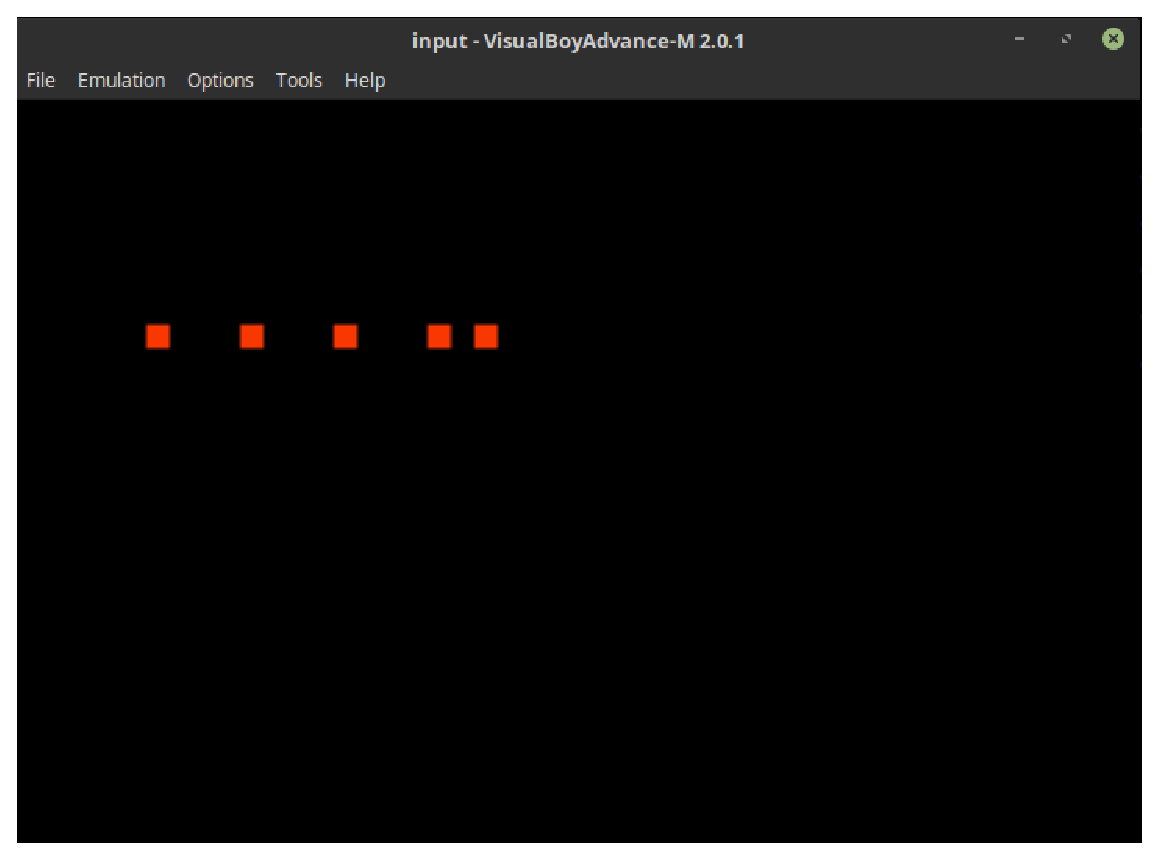
\includegraphics[keepaspectratio=true,scale=0.6]{figuras/demo-input.eps}
   \caption[Demonstração do pressionamento de botões no emulador]
    {Teste de pressionamento de botões no emulador. Fonte: \textit{Autores}.}
   \label{demo-input}
\end{figure}

\begin{lstlisting}[float,caption={Código de teste de \textit{input}.},label={lst:inputtest}]
#include "video.h"
#include "input.h"

#define RED 0x0000FF

unsigned short *vid_mem = (unsigned short *)0x6000000;

int main() {
    reset_dispcnt();
    set_video_mode(3);
    set_background_number(2);

    while(1) {
        check_buttons_states();

        for(int i=0;i<=9;i++){
            if (pressed(i)) {
                vid_mem[50 * 240 + i * 10] = RED;
            } else {
                vid_mem[50 * 240 + i * 10] = 0;
            }
        }
    }

    return 0;
}
\end{lstlisting}

O código deste projeto se enconra no seguinte endereço \url{https://github.com/traveling-will-gba/gbengine/tree/dev/test/input}.